% Hanrich Potgieter		
% Check 
The system should be able to easily address future integration requirements by providing access to its services using widely adopted public standards.
\subsubsection*{Integratability A}
Notification A is not integratable beacuse of the following reasons.
\begin{itemize}
	\item \textbf{Installing required Packages.}
	There is no way of installing the required packages. This degrades the qualitly of the integratability of the system as one has to manually figure out which packages to include in the system.
	\item \textbf{Dependancy Injection}
	There is no dependacy injection.
	\item \textbf{Unit tests}
	There was no supplied unit test. Unit test are xritical to determin wheater or not we can integrate it into a lager system.
\end{itemize}
\subsubsection*{Integratability B}
The integratability of notification B is not adequite. There are numerbour challanges that are missing. There is no dependancy injection and all packages needs to be installed manually.
\begin{itemize}
	\item {File Structure} 
	Each function is placed in a seperate file. There is no common module to integrate that will allow access to all the capabilities of notifications.
	\item Installing required packages
	One cannot easily install the dependancys that is required by Notifications.
	\item Dependancy Injection.
	There is no dependacy injection.
	\item
	Inappropriate Unit testing. Therefore we cannot test if the functions is working. There is a file called test.js that is an attempt at unit testing but no proper unit testing was applied. They should have used someting similar to Unit.js with mocha.
		~\ref{fig:IntegrationUnitTest}
		\begin{figure}[H]
			\centering
			\fbox{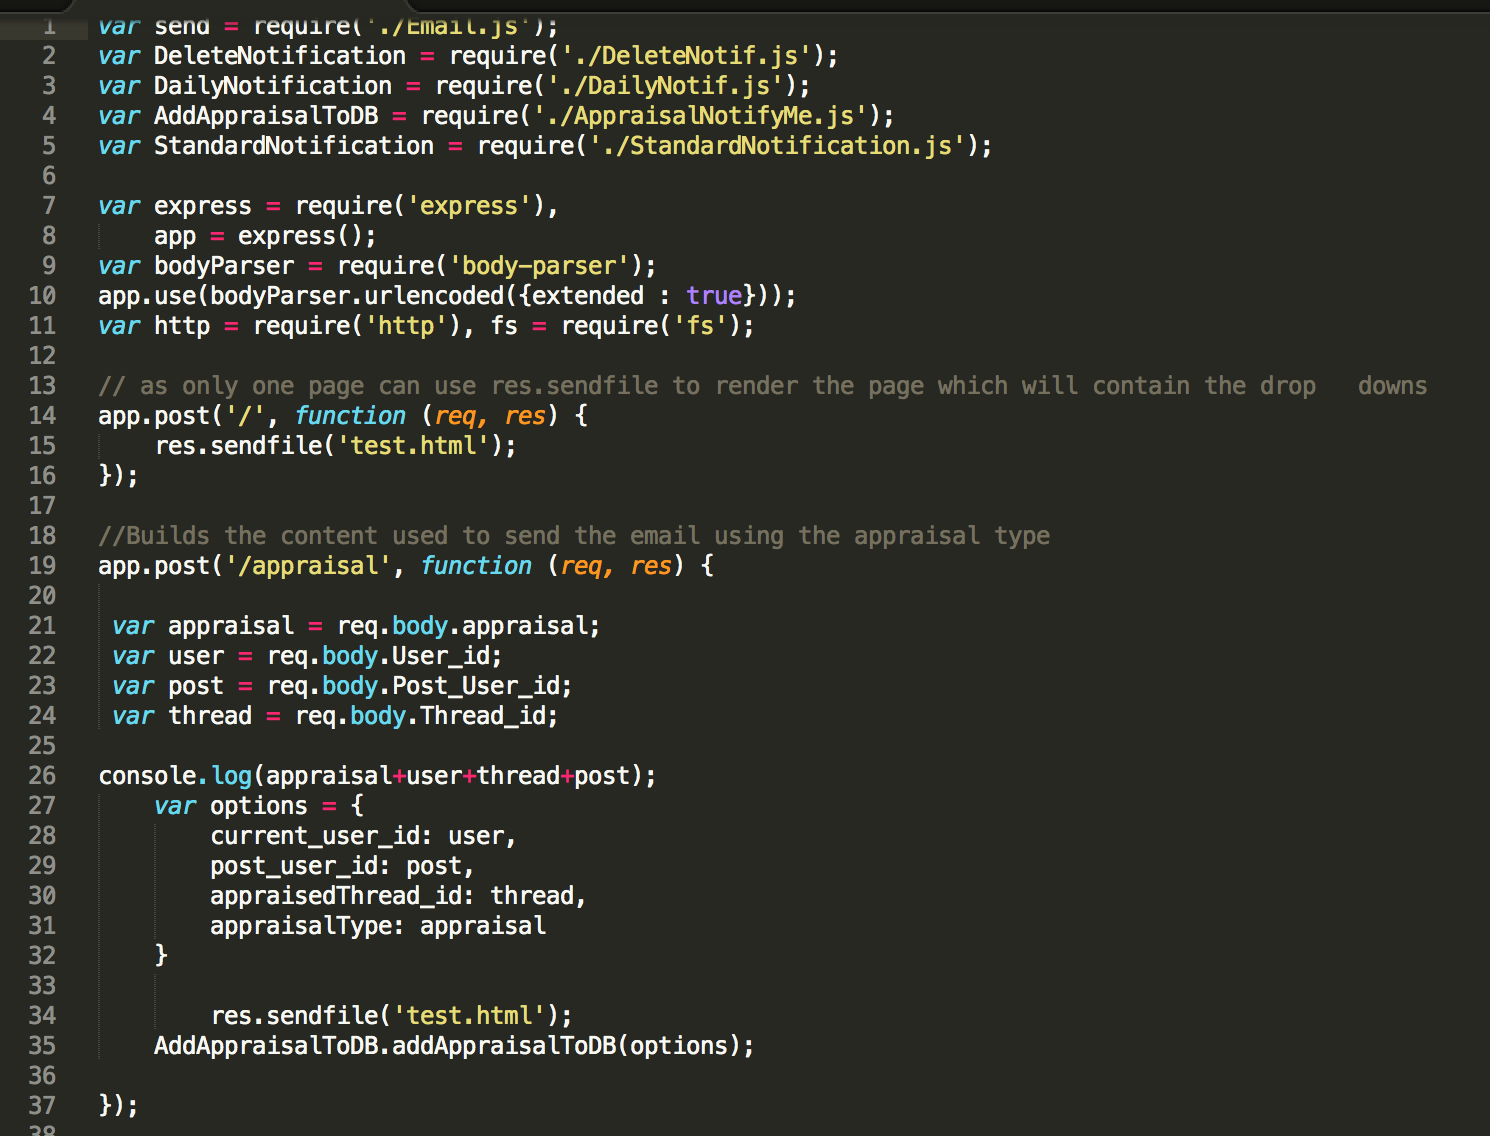
\includegraphics[width=1.0\textwidth]{IntegrationUnitTest}}
			\caption{Unit Tests}
			\label{fig:scope}
		\end{figure}
	\item database issues
	There is no way to access the specified database and this also contributes to the integratability. They sould supply a way to specifiy the database to be used.
		~\ref{fig:IntegrationDatabaseFail}
		\begin{figure}[H]
			\centering
			\fbox{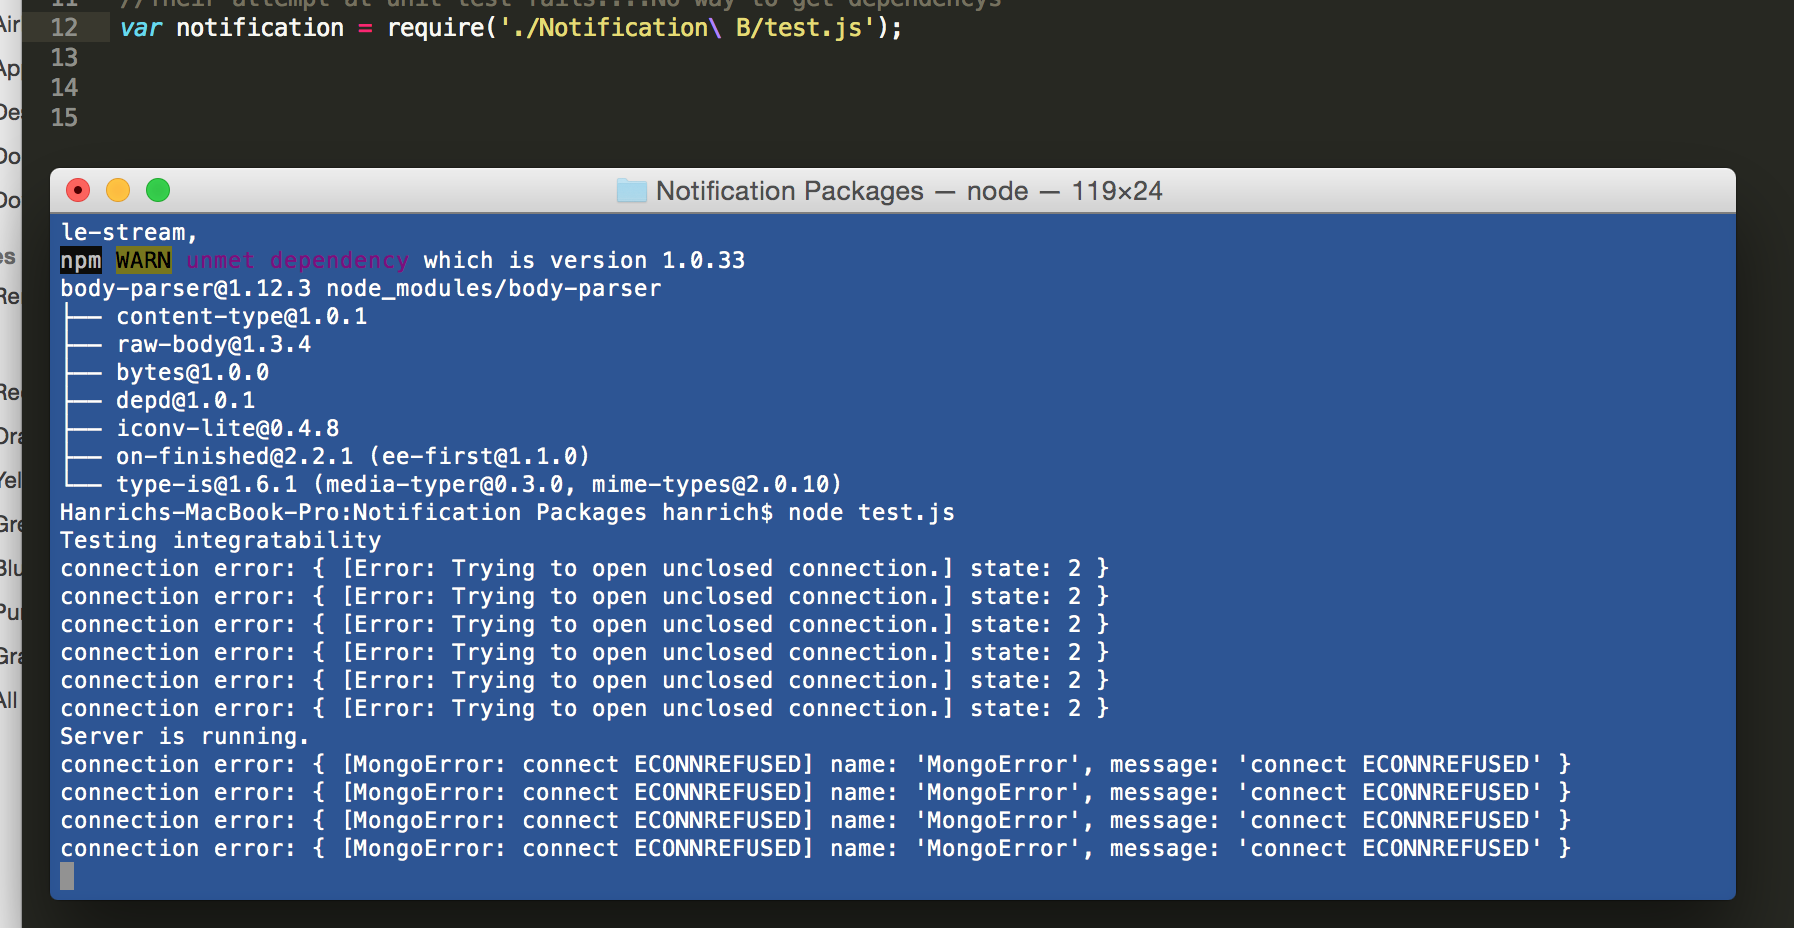
\includegraphics[width=1.0\textwidth]{IntegrationDatabaseFail}}
			\caption{Database connection issues}
			\label{fig:scope}
		\end{figure}
\end{itemize}
\subsubsection*{Remarks}
Notification B is not Integratable at alll. There is no provision for dependacny injection.